% *********************************************************************
% © 2021–2026 Jeremy Sylvestre
%
% Permission is granted to copy, distribute and/or modify this document
% under the terms of the GNU Free Documentation License, Version 1.3 or
% any later version published by the Free Software Foundation; with no
% Invariant Sections, no Front-Cover Texts, and no Back-Cover Texts. A
% copy of the license is included in the appendix entitled “GNU Free
% Documentation License” that appears in the output document of this
% PreTeXt source code. All trademarks™ are the registered® marks of
% their respective owners.
%
% *********************************************************************

\newcommand*{\xmin}{-6.25}
\newcommand*{\xmax}{10.25}
\newcommand*{\ymin}{-1.5}
\newcommand*{\ymax}{1.5}

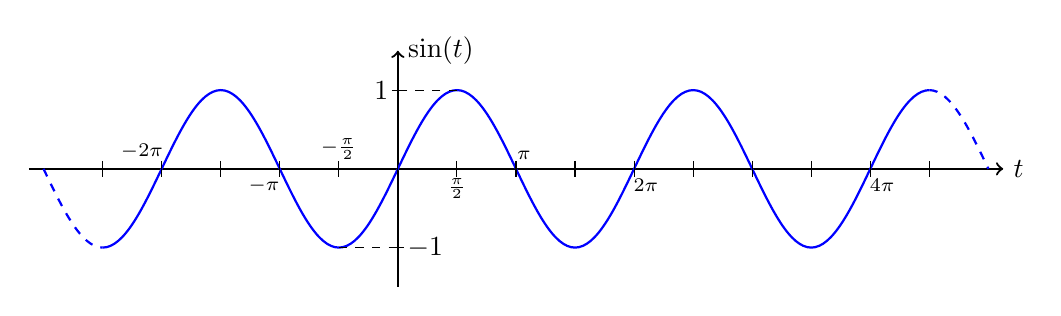
\begin{tikzpicture}
[
	closedpt/.style={circle,draw,fill,inner sep=0pt,minimum size=4pt},
	openpt/.style={circle,draw,inner sep=0pt,minimum size=4pt},
	xscale=0.75
]

	% axes
	\draw[->,thick] (\xmin,0) -- (\xmax,0) node[right] {$t$};
	\draw[->,thick] (0,\ymin) -- (0,\ymax) node[right] {$\sin(t)$};

	\draw[blue,thick,dashed] (-6,0) sin (-5,-1);
	\draw[blue,thick,dashed] (9,1) cos (10,0);

	\draw[blue,thick]
	  (-5,-1)
	  cos (-4,0)
	  sin (-3,1)
	  cos (-2,0)
	  sin (-1,-1)
	  cos (0,0)
	  sin (1,1)
	  cos (2,0)
	  sin (3,-1)
	  cos (4,0)
	  sin (5,1)
	  cos (6,0)
	  sin (7,-1)
	  cos (8,0)
	  sin (9,1)
	;

	\foreach \x in {-5,-4,-3,...,9} {
		\draw (\x,0.1) -- (\x,-0.1);
	}

	\node[above,xshift=-0.25cm] at (-4,0) {$\scriptstyle -2 \pi$};
	\node[below,xshift=-0.2cm] at (-2,0) {$\scriptstyle - \pi$};
	\node[above] at (-1,0) {$\scriptstyle - \frac{\pi}{2}$};

	\node[below] at (1,0) {$\scriptstyle \frac{\pi}{2}$};
	\node[above,xshift=0.1cm] at (2,0) {$\scriptstyle \pi$};
	\node[below,xshift=0.15cm] at (4,0) {$\scriptstyle 2 \pi$};
	\node[below,xshift=0.15cm] at (8,0) {$\scriptstyle 4 \pi$};

	\draw[dashed] (1,1) -- (0,1) node[left] {$1$};
	\draw[dashed] (-1,-1) -- (0,-1) node[right] {$-1$};
	\foreach \y in {-1,1} {
		\draw (-0.1,\y) -- (0.1,\y);
	}

\end{tikzpicture}
